\termin{20.05.2016}

\mdf{Satz}
Jede \textit{reelle} Couchy-Folge ist konvergent.

\mdf{Definition}
Sei $D \subseteq \mathbb{R}, f : D \rightarrow \mathbb{R}$ eine Abbildung und $x_0 \in \mathbb{R}$. Gilt für jede Folge $x_n \in D$ mit $\lim\limits_{n \to \infty}x_n = x_0$ dass $\lim\limits_{n \to \infty}f(x_n) = y_0$, dann heißt $y_0$ der \begr[Grenzwert]{Grenzwert von f(x) für $x$ gegen $x_0$}. Kurz:
\begin{align*}
	\lim\limits_{n \to \infty}f(x) = y_0
\end{align*}
Für Grenzwerte von Abbildungen gilt Satz 7 analog.

\mdf{Beispiel}
Sei
\begin{align*}
	&f : \mathbb{R} \rightarrow \mathbb{R} \\
	&x \mapsto x^2
\end{align*}
und $x_0 \in \mathbb{R}$ beliebig aber fest, sowie $x_n$ eine beliebige Folge, die gegen $x_0$ konvergiert. Dann:
\begin{align*}
	\lim\limits_{n \to \infty}f(x_n) &= \lim\limits_{n \to \infty}x_n^2 = \left(\lim\limits_{n \to \infty}x_n\right)\left(\lim\limits_{n \to \infty}x_n\right) \\
	&= x_0^2 = f(x_0) = y_0
\end{align*}
Also:
\begin{align*}
	\lim\limits_{x \to x_0}f(x) = y_0
\end{align*}

Sei
\begin{align*}
	&g : \mathbb{R} \rightarrow \mathbb{R} \\
	&x \mapsto \begin{cases}
		1 & x \geq 0 \\
		0 & x < 0
	\end{cases}
\end{align*}
und $x_n$ eine nicht negative Nullfolge. Dann gilt
\begin{align*}
	\lim\limits_{n \to \infty}g(x_n) = \lim\limits_{n \to \infty}1 = 1 = f(x_0)
\end{align*}
Sei aber $x_n$ eine negative Nullfolge.
\begin{align*}
	\lim\limits_{n \to \infty}g(x_n) = \lim\limits_{n \to \infty}0 = 0 \neq f(x_0)
\end{align*}
Das heißt der Grenzwert von $f(x)$ für $x$ gegen $x_0$ existiert nicht.

\mdf{Definition}
Sei $D \subseteq \mathbb{R}, f : D \rightarrow \mathbb{R}$ eine Abbildung. $f$ heißt \begr[Stetigkeit, Stelle]{stetig an der Stelle} $x_0 \in D$, falls gilt:
\begin{align*}
	\lim\limits_{x \to x_0}f(x) = f(x_0)
\end{align*}
Ist $f$ stetig an jedem Punkt $x_0 \in D$, so heißt $f$ \begr[Stetigkeit]{stetig auf $D$}.

\mdf{Satz} ($\varepsilon{}$--$\delta{}$--Stetigkeit)

Sei $D \subseteq \mathbb{R}, f : D \rightarrow \mathbb{R}$ eine Abbildung. $f$ ist an der Stelle $x_0 \in D$ genau dann stetig, wenn gilt:
\begin{align*}
	\forall \varepsilon > 0\enspace\exists\,\delta > 0 : |x - x_0| < \delta \Rightarrow |f(x) - f(x_0)| < \varepsilon
\end{align*}

\begin{center}
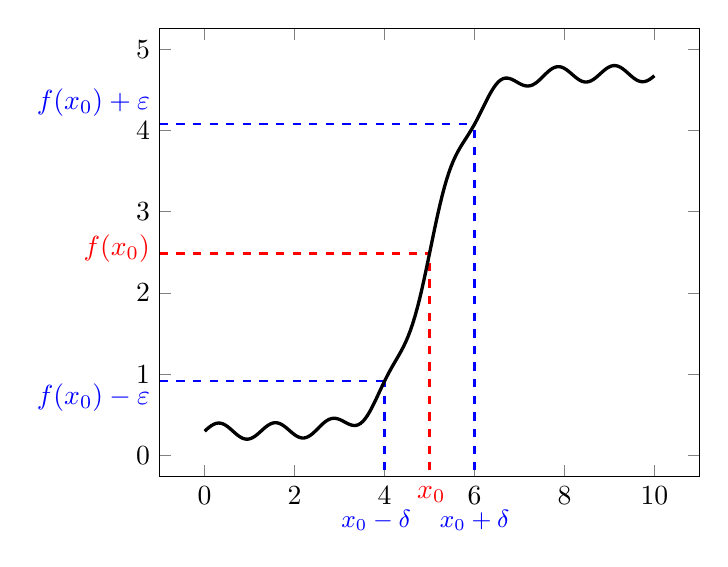
\begin{tikzpicture}[font=\sffamily]
\begin{axis}[samples=200,domain=0:10,restrict y to domain =0:10]
	\draw [red, dashed, thick] (axis cs:5,-1) -- (axis cs:5,2.486);
	\draw [red, dashed, thick] (axis cs:-1,2.486) -- (axis cs:5,2.486);
	
	\draw [blue, dashed, thick] (axis cs:-1,0.916) -- (axis cs:4,0.916);
	\draw [blue, dashed, thick] (axis cs:4,-1) -- (axis cs:4,0.916);
	
	\draw [blue, dashed, thick] (axis cs:-1,4.077) -- (axis cs:6,4.077);
	\draw [blue, dashed, thick] (axis cs:6,-1) -- (axis cs:6,4.077);
	
	\addplot[very thick,black] plot (\x, {2.2*tanh((\x)-5)+2.5+sin(5*\x r)*0.1});
\end{axis}
\node [below, red] at (3.45,0) {$x_0$};
\node [left, red] at (0,2.9) {$f(x_0)$};

\node [below, blue] at (2.75,-0.3) {\small$x_0 - \delta$};
\node [left, blue] at (0,1) {$f(x_0) - \varepsilon$};

\node [below, blue] at (4,-0.3) {\small$x_0 + \delta$};
\node [left, blue] at (0,4.75) {$f(x_0) + \varepsilon$};

\end{tikzpicture}
\end{center}

\mdf{Beispiel}
Sei $f : \mathbb{R} \rightarrow \mathbb{R}\quad f(x) = 5x^2 + 2x - 1,\quad x_0 = 0$. Das heißt, wir suchen für jedes $\varepsilon > 0$ ein $\delta$ das den Satz erfüllt.
\begin{align*}
	|f(x) - f(x_0)| = |5x^2 + 2x| \leq 5|x|^2 + 2|x|\text{ und }|x - x_0| = |x|
\end{align*}
Wir müssen $\delta$ so wählen, dass $5\delta{}^2 + 2\delta{} < \varepsilon$. Wähle $\delta$ so, dass $\delta < 1$ und $\delta < \frac{\varepsilon}{7}$. Dann gilt für alle $x \in \mathbb{R}$ mit $|x - x_0| = |x| < \delta$:
\begin{align*}
	|f(x) - f(x_0)| \leq 5|x|^2 + 2|x| < 5\delta{}^2 + 2\delta{} < 7\delta{}
\end{align*}
Da $\delta{} < 1$ gilt ist $5\delta{}^2 + 2\delta{} < 7\delta{}$.

\mdf{Satz}
Jedes Polynom
\begin{align*}
	f : \mathbb{R} \rightarrow \mathbb{R}, f(x) = \sum_{i = 0}^{n} a_ix^i
\end{align*}
ist stetig auf $\mathbb{R}$.

\bigskip\textbf{Beweis:}

\begin{enumerate}
	\item{
		Über Grenzwerte. Sei $x_0 \in \mathbb{R}$ beliebig und $x_k$ eine Folge die gegen $x_0$ konvergiert. Nach Satz 7:
		\begin{align*}
			\lim\limits_{k \to \infty}f(x_k) = \sum_{i = 0}^{n}\left(a_i \lim\limits_{k \to \infty}x_k^i\right) = \sum_{i = 0}^{n}\left(a_i \lim\limits_{k \to \infty}x_k\right)^i = \sum_{i = 0}^{n} a_ix_0^i = f(x_0)
		\end{align*}
		Da $x_k$ beliebig war, gilt $\lim\limits_{x \to x_0}f(x) = f(x_0)$. Also ist $f$ in $x_0$ stetig. Da $x_0 \in \mathbb{R}$ beliebig war, ist $f$ stetig auf $\mathbb{R}$.
	}
	\item{
		Über $\varepsilon{}$--$\delta{}$--Kriterium. Sei also $x_0 \in \mathbb{R}$ beliebig und $\varepsilon > 0$. Wir setzen
		\begin{align*}
			\delta = \text{min}\left\{1,\frac{\varepsilon}{n\cdot\text{max}\left\{|a_i|(|x_0|+1)^{i-1}\right\}}\right\}
		\end{align*}
		Aus $\delta = 1$ folgt für $x \in \mathbb{R}$ mit $|x - x_0| < \delta$:
		\begin{align*}
			|x| = |x - x_0 + x_0| \leq |x - x_0| + |x_0| < \delta{}+|x_0| \leq |x_0|+1
		\end{align*}
		Also:
		\begin{align*}
			&|f(x) - f(x_0)| \leq \sum_{i=1}^{n}|a_i|\cdot (x^i - x_0^i) = \sum_{i=1}^{n}|a_i|\left|\sum_{l=0}^{i-1}(x_0 - x)x_0x^{i-1-l}\right| < \delta \sum_{i=0}^{n} |a_i|\sum_{l=0}^{i-1} |x_0|^l |x|^{i-1-l} \\
			&|x_0|^l |x|^{i-1-l} < (|x_0|+1)^l(|x_0|+1)^{i-1-l} = (|x_0|+1)^{i-1}
		\end{align*}
		Wegen $\delta \leq \frac{\varepsilon}{n\cdot\text{max}\left\{|a_i|(|x_0|+1)^{i-1}\right\}}$ folgt:
		\begin{align*}
			|f(x)-f(x_0)| < \delta{}\sum_{i=0}^{n}|a_i|\sum_{l=0}^{i-1}(|x_0|+1)^{i-1} \leq \delta \cdot n \cdot \text{max}\left\{|a_i|(|x_0|+1)^{i-1}\right\} \leq \varepsilon
		\end{align*}
	}
\end{enumerate}

\mdf{Satz}
Sind $g, h : \mathbb{R} \rightarrow \mathbb{R}$ Polynome, so ist $f(x) = \frac{g(x)}{h(x)}$ stetig an jeder Stelle, an der $f$ definiert ist ($h(x) \neq 0$).

Die bekannten Abbildungen $\text{sin}, \text{cos}, \text{tan}, \text{exp}$ sind stetig auf $\mathbb{R}$.



